\PassOptionsToPackage{unicode,pdfusetitle}{hyperref}
\PassOptionsToPackage{hyphens}{url}
\PassOptionsToPackage{dvipsnames,svgnames,x11names}{xcolor}

\documentclass[10pt]{beamer}

\usetheme{moloch}
\usefonttheme{professionalfonts}
\setbeamertemplate{page number in head/foot}[appendixframenumber]

\usepackage{lmodern}
\usepackage{amssymb,amsmath,mathtools,amsthm}
\usepackage[T1]{fontenc}
\usepackage{textcomp}

\usepackage{upquote} % straight quotes in verbatim environments
\usepackage{microtype}
\UseMicrotypeSet[protrusion]{basicmath} % disable protrusion for tt fonts

\usepackage{xcolor}
\usepackage{xurl} % add URL line breaks if available
\usepackage{bookmark}
\usepackage{hyperref}

\hypersetup{%
  colorlinks = true,
  linkcolor  = mLightGreen,
  filecolor  = mLightGreen,
  citecolor  = mLightGreen,
  urlcolor   = mLightGreen
}

%% subfigures
% \usepackage{subcaption}

% % algorithms
% \usepackage[ruled,vlined]{algorithm2e}
% \resetcounteronoverlays{algocf}

\usepackage{booktabs}

\date{\today}
\titlegraphic{
\includegraphics{figures/logo.pdf}}


% % bibliography
% \usepackage[style=authoryear]{biblatex}
% \addbibresource{uppsala.bib}

% title block
\title{Fjasdf}
\subtitle{Subtitle}
\author{Johan Larsson}
\institute{Department of Statistics, Lund University}

% operators
\DeclareMathOperator*{\argmax}{arg\,max}
\DeclareMathOperator*{\argmin}{arg\,min}
\DeclareMathOperator{\E}{E}
\DeclareMathOperator{\var}{Var}
\DeclareMathOperator{\cov}{Cov}
\DeclareMathOperator{\tr}{tr}
\DeclareMathOperator{\diag}{diag}
\DeclareMathOperator{\range}{range}
\DeclareMathOperator{\nullspace}{null}
\DeclareMathOperator{\rank}{rank}
\DeclareMathOperator{\card}{card}
\DeclareMathOperator{\sign}{sign}
\DeclareMathOperator{\st}{S}
\DeclareMathOperator{\normal}{Normal}
\DeclareMathOperator{\fnormal}{FoldedNormal}
\DeclareMathOperator{\bernoulli}{Bernoulli}
\DeclareMathOperator{\erf}{erf}
\DeclareMathOperator{\mse}{MSE}
\DeclareMathOperator{\risk}{R}
% \DeclareMathOperator{\I}{I}
% \DeclareMathOperator{\T}{}
%
% \DeclareMathSymbol{\phi}{\mathalpha}{operators}{0}
\DeclareMathOperator{\pdf}{\phi}
\DeclareMathOperator{\cdf}{\Phi}
% commands
% \newcommand{\vec}{\vectorsym}
% \newcommand{\mat}{\matrixsym}
\renewcommand{\vec}{\boldsymbol}
\newcommand{\mat}{\boldsymbol}
\newcommand*\du{\mathop{}\!\mathrm{d}}
% \newcommand{\T}{\mathsf{T}}
\newcommand{\T}{\intercal}
\newcommand{\ones}{\boldsymbol{1}}
% \newcommand{\T}{\intercal}
% \newcommand{\T}[1]{{1}^{\mathsf{T}}}
\newcommand{\ind}[1]{\operatorname{I}_{#1}}

% environments
\theoremstyle{plain}
\newtheorem{theorem}{Theorem}[section]
\newtheorem{corollary}{Corollary}[theorem]
\newtheorem{lemma}{Lemma}[section]
\newtheorem{proposition}{Proposition}[section]

\theoremstyle{definition}
\newtheorem{definition}{Definition}[section]
\newtheorem{example}{Example}[section]

\theoremstyle{remark}
\newtheorem{remark}[theorem]{Remark}

\newcommand{\todojl}[1]{\todo[color=green!40]{#1}}




\begin{document}

\maketitle

% \begin{frame}
%   \frametitle{Overview}
%
%   \tableofcontents
% \end{frame}

\section{Preliminaries}

\begin{frame}
  \frametitle{General Setup}

  \begin{itemize}
    \item Data consists of a \alert{fixed} matrix of features \(\mat{X} \in \mathbb{R}^{n \times p}\) and a response vector \(\vec{y} \in \mathbb{R}^n\).
    \item \(\vec{y}\) comes from a linear model, that is,
          \[
            y_i = \beta_0^* + \vec x_i^\T \vec\beta^* + \varepsilon_i \quad\text{for} \quad i \in 1,\dots,n,
          \]
          where \(\vec{\beta}^*\) is the vector of \emph{true} coefficients.
    \item \(\varepsilon_i\) is the measurement noise, generated from some random variable\footnote{No assumption on normality (yet).}.
  \end{itemize}
\end{frame}

\begin{frame}[c]
  \frametitle{The Elastic Net}

  Linear regression plus a combination of the \(\ell_1\) and \(\ell_2\) penalties:
  \begin{equation*}
    \hat{\vec{\beta}} = \argmin_{\beta \in \mathbb{R}^p} \left( \frac{1}{2} \lVert \vec y - \beta_0 - \tilde{\mat{X}}\vec{\beta} \rVert^2_2  + \lambda_1 \lVert \vec\beta \rVert_1 + \frac{\lambda_2}{2}\lVert \vec \beta \rVert_2^2\right).
  \end{equation*}

  \pause

  % \begin{block}{Special Cases}
  %   \begin{description}[Lasso]
  %     \item[OLS] \(\lambda_1 = \lambda_2 = 0\)
  %     \item[Lasso] \(\lambda_1 > 0\) and \(\lambda_2 = 0\)
  %     \item[Ridge] \(\lambda_1 = 0\) and \(\lambda_2 > 0\)
  %   \end{description}
  % \end{block}

  \begin{figure}
    \centering
    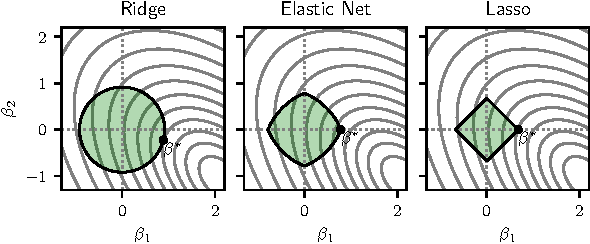
\includegraphics[]{figures/elasticnet-balls.pdf}
    \caption{%
      The elastic net penalty is a combination of the lasso and ridge penalties
    }
  \end{figure}

  % TODO: Insert figure of elastic net, ridge, lasso here. Possibly just the constraint regions?
\end{frame}

\begin{frame}[c]
  \frametitle{Sensitivity to Scale}

  Since both the lasso and ridge penalties are norms, they are sensitive to the scale of the input features.

  \medskip

  But what is the \emph{optimal} scaling?

  \medskip

  If the features are ``normal'', then most people would agree that stanardizing them (i.e., subtracting the mean and dividing by the standard deviation) is a good idea.
\end{frame}

\begin{frame}[c]
  \frametitle{Normalization}

  Let \(\mat S\) be the \emph{scaling matrix}, which is a \(p \times p\) diagonal matrix with entries \(s_1, s_2, \dots, s_p\). Let \(\mat C\) be the \emph{centering matrix}, which is an \(n \times p\) matrix with each row equal to \([c_1, c_2, c_n]^\T\). Then the \emph{normalized design matrix} \(\tilde{\mat X}\) is defined as \(\tilde{\mat X} = (\mat X - \mat C)\mat S^{-1}\).
\end{frame}

\begin{frame}[c]
  \begin{table}[hbt]
    \centering
    \caption{Common ways to normalize a matrix of features}
    \label{tab:normalization-types}
    \begin{tabular}{lll}
      \toprule
      Normalization    & Centering (\(c_{1j}\))             & Scaling (\(s_j\))                                         \\
      \midrule
      Standardization  & \(\frac{1}{n}\sum_{i=1}^n x_{ij}\) & \(\sqrt{\frac{1}{n}\sum_{i=1}^n (x_{ij} - \bar{x}_j)^2}\) \\
      \addlinespace
      Min--Max         & \(\min_i(x_{ij})\)                 & \(\max_i(x_{ij}) - \min_i(x_{ij})\)                       \\
      \addlinespace
      Unit Vector (L2) & 0                                  & \(\sqrt{\sum_{i=1}^n x_{ij}^2}\)                          \\
      \addlinespace
      Max--Abs         & 0                                  & \(\max_i(|x_{ij}|)\)                                      \\
      \addlinespace
      Adaptive Lasso   & 0                                  & \(\beta_j^\text{OLS}\)                                    \\
      \bottomrule
    \end{tabular}
  \end{table}
\end{frame}

\begin{frame}[c]
  \frametitle{Binary Features}

  Let's say we have a binary feature \(\vec{x}_j\), such that \(x_{ij} \in \{0, 1\}\).

  \medskip

  What is the ``best'' way to scale this feature?

\end{frame}

\begin{frame}[c]
  \frametitle{Solution for Binary Features}

  We assume the that normalized features are orthogonal, that is
  \[
    \tilde{\mat{X}}^\T \tilde{\mat{X}} = \diag(\dots)
  \]
\end{frame}

\begin{frame}[c]
  \frametitle{Class Imbalance}

\end{frame}

\section{Mixed Data}

\begin{frame}[c]
  \frametitle{Mixed Data}

\end{frame}

\section{Experiments}


% \begin{frame}[standout]
%   Thank you!
% \end{frame}

% \appendix
% 
% \begin{frame}[allowframebreaks]{References}
%   \printbibliography[heading=none]
% \end{frame}

\end{document}

